%%
%% Author: dariochinelli
%% 2021-04-03
%%


\section{Il corpo nero}
Il corpo nero è un concetto utile per descrivere un oggetto le cui pareti si trovino a temperatura $T$ uniforme e costante, esso emette uno spettro di radiazione continuo che dipende solamente dalla temperatura e non dal materiale di cui è composto.
Le cariche elettriche costituenti le pareti si muovono in virtù dell'agitazione termica e così facendo irraggiano onde elettromagnetiche che vanno riempiendo la cavità: in questo modo si trasferisce energia dalle pareti al campo elettromagnetico al suo interno.
Tali onde elettromagnetiche a loro volta urtando contro le pareti trasferiscono energia dal campo elettromagnetico alle pareti.
Quando si raggiunge l'equilibrio termico tra le onde all'interno e le pareti dell'oggetto si ha che l'energia ricevuta è uguale a quella emessa.\\
\textbf{Definiamo} \\
\underline{\textit{Radianza Spettrale}}: $R_T(\nu)$ potenza su area, ovvero energia emessa per unità di tempo nell'intervallo di frequenze tra $\nu$ e $\nu+d\nu$ da un'area unitaria di superficie ad una certa temperatura $T$. \\
\underline{\textit{Radianza Totale} o \textit{Radianza}}: $R_T= \int_0^{\infty} R_T(\nu)d\nu$ integrale su tutte le frequenze della radianza spettrale, descrive l'energia totale per unità di tempo di un'area unitaria di superficie ad una certa temperatura $T$.
\begin{figure}[h]
\centering
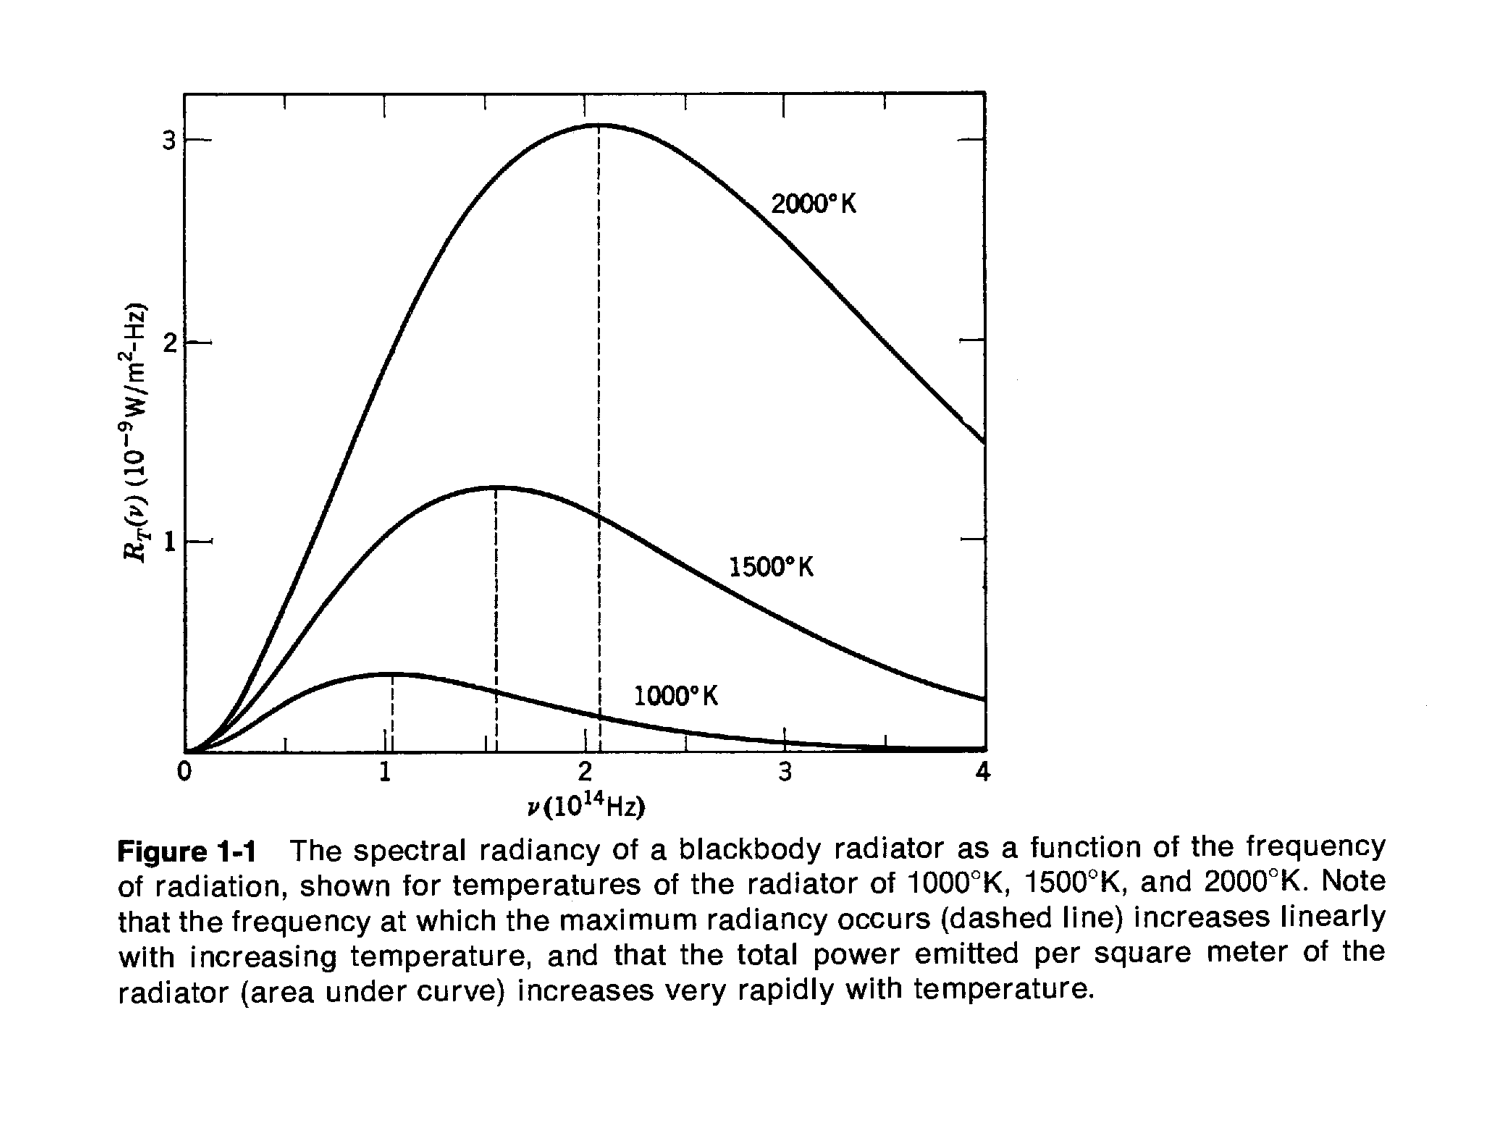
\includegraphics[scale=0.6]{/Spectral_radiancy}
\caption{Radianza spettrale di corpo nero a tre diverse temperature. Notare come il picco si sposti all'aumentare della temperatura.}
\end{figure}
Per descrivere la radiazione di corpo nero Rayleigh e Jeans utilizzarono (anche) le seguenti leggi empiriche:
la \textbf{legge di Stefan-Boltzmann}:
\begin{equation}
R_T = \sigma T^4
\end{equation}
che descrive la radianza totale in funzione della temperatura ed in cui compare la 
\begin{equation}
\mbox{\underline{costante di Stefan-Boltzmann}} \quad \sigma = 5.67 \cdot 10^{-8} \frac{W}{m^2 \cdot K^4}
\end{equation}
La \textbf{legge di spostamento di Wien} afferma che la frequenza di picco è proporzionale alla temperatura
\begin{equation}
\begin{split}
& \nu_{max} \propto T \\
& \mbox{ed usando la seguente relazione} \quad \lambda\nu = c \\
& \lambda_{max}T = \SI{2.898e-3}{mK}
\end{split}
\end{equation}
L'oggetto reale più simile al concetto teorico di corpo nero è la \underline{cavità di corpo nero}, cioè un oggetto cavo con pareti metalliche avente un piccolo buco sulla superficie: la radiazione che esce dal foro è interpretabile come corpo nero, vedi figura.
\begin{figure}[h]
\centering
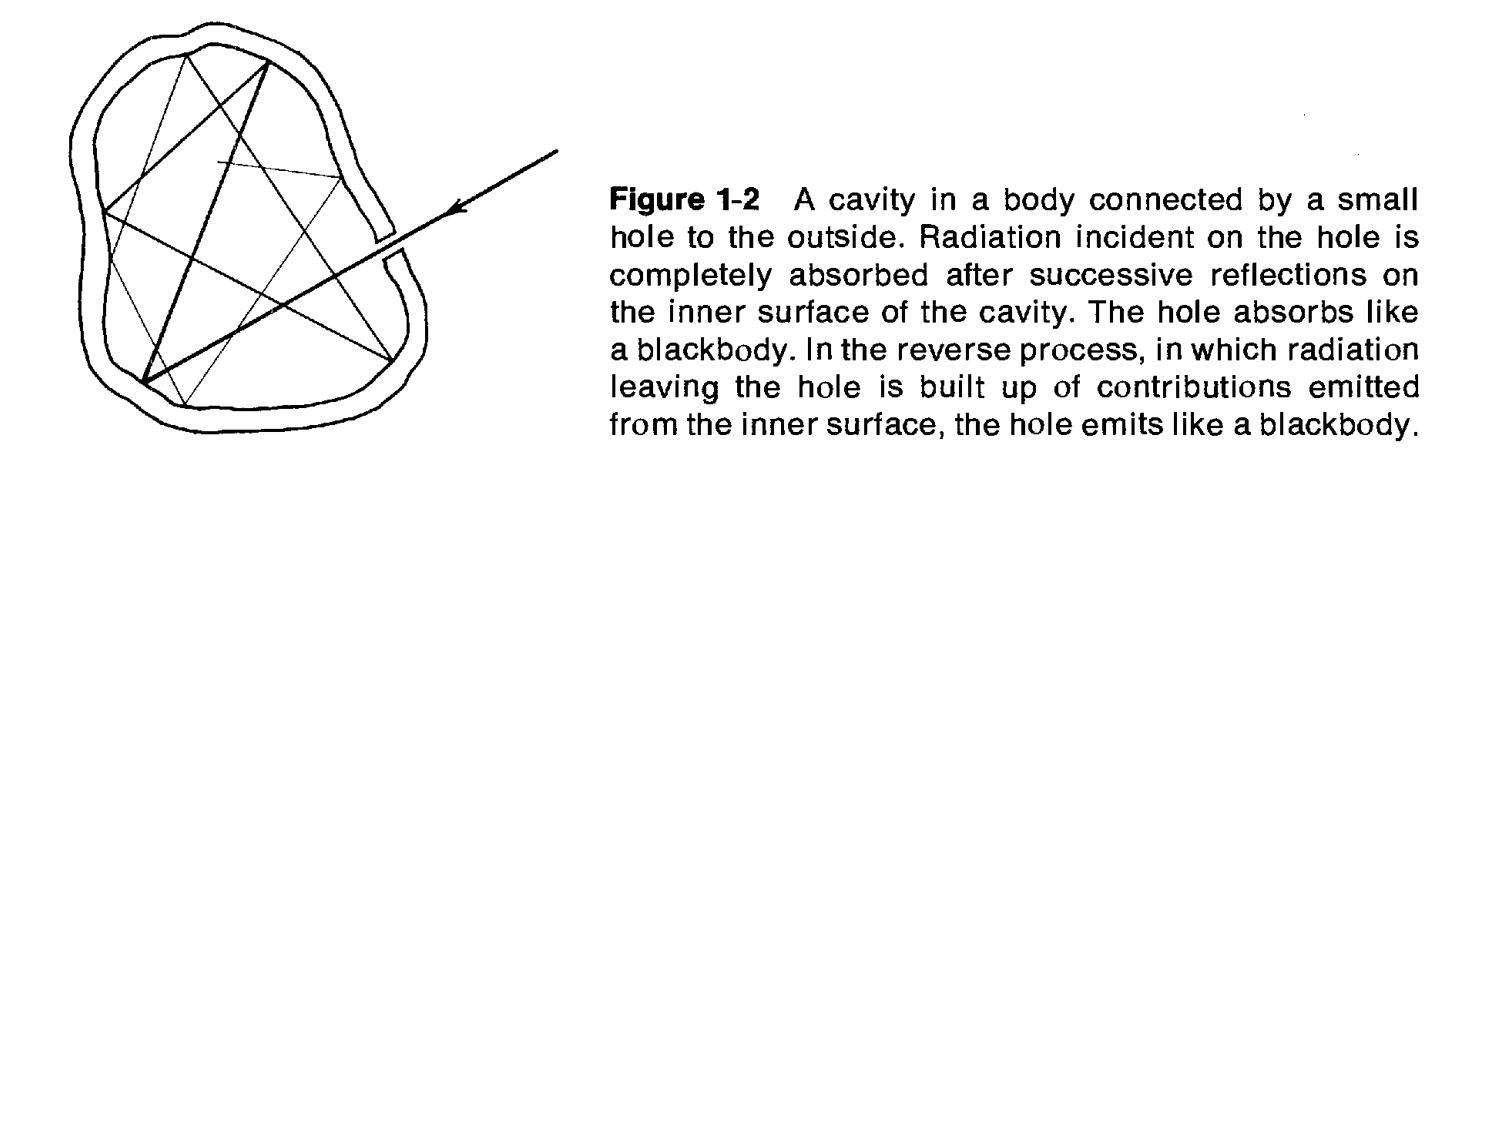
\includegraphics[scale=0.6]{/cavita_corponero}
\end{figure}
Introduciamo la \underline{\textbf{radiazione di cavità}} $\rho_T(\nu)$, che è la densità di energia contenuta in una unità di volume della cavità ad una certa temperatura $T$,
essa è ovviamente proporzionale alla Radianza totale, la cui derivazione è basata su ragionamenti puramente geometrici, in particolare la relazione è data da:
\begin{equation}
\frac{c}{4}\rho_T(\nu)=R_T(\nu)
\end{equation}


\subsection{Teoria classica di corpo nero di Rayleigh e Jeans}
A inizio '900 spiegare la forma dello spettro di corpo nero era uno dei problemi più dibattuti.
A dare un grande contributo furono Rayleigh e Jeans, che elaborarono la teoria classica di corpo nero, basandosi sulla fisica classica, per modellizzare la forma dello spettro di corpo nero.
Quindi si impegnarono nel trovare un modello teorico che potesse spiegare i risultati sperimentali. \\
Il ragionamento si divide in tre passaggi:
\begin{enumerate}[label=\Roman{*}.]
\item Le onde elettromagnetiche all'interno della cavità sono onde stazionarie?
\item Come contare il numero di onde stazionarie?
\item È possibile associare un'energia alle onde elettromagnetiche?
\end{enumerate}
\begin{figure}[h]
\centering
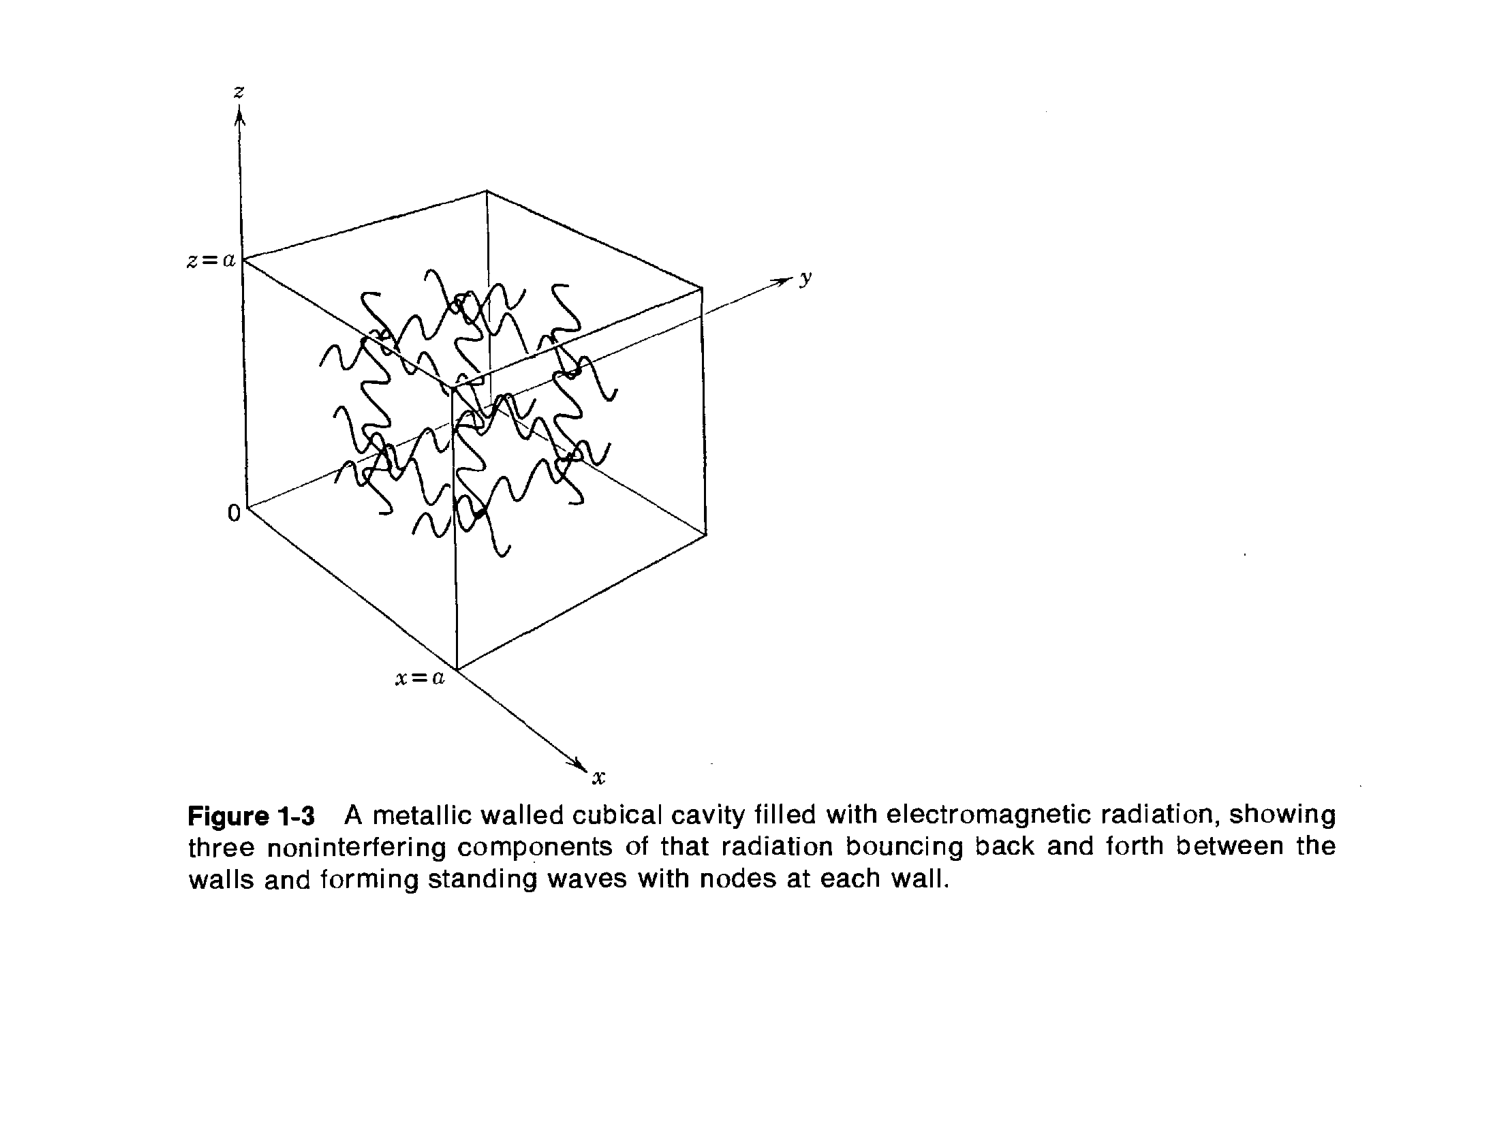
\includegraphics[scale=0.7]{/cubo_CorpoNero}
\caption{cubo Corpo Nero}
\end{figure}
Si consideri una cavità cubica e metallica riscaldata a temperatura $T$.
Essi ragionarono con le frequenze delle onde elettromagnetiche contenute nella cavità.
Vediamo in dettaglio i passaggi seguiti da Rayleigh e Jeans.
\begin{enumerate}[label=\Roman{*}.]
\item Prima di tutto occorre dimostrare che tali onde siano stazionarie.
Ogni onda può essere scomposta lungo le tre componenti spaziali e studiata indipendentemente. 
Consideriamo il lato del cubo $x \in (0, a)$.
La radiazione elettromagnetica è trasversale, cioè il campo elettrico $\vec{E}$ è perpendicolare alla direzione di propagazione dell'onda, dunque il campo è parallelo alla parete, ma ciò porta all'annullarsi di $\vec{E}$ sulla parete, perciò sui lati del cubo deve esserci ampiezza nulla, e quindi $0$ e $a$ sono due nodi.
Le onde sono dunque stazionarie.
\begin{figure}[h]
\centering
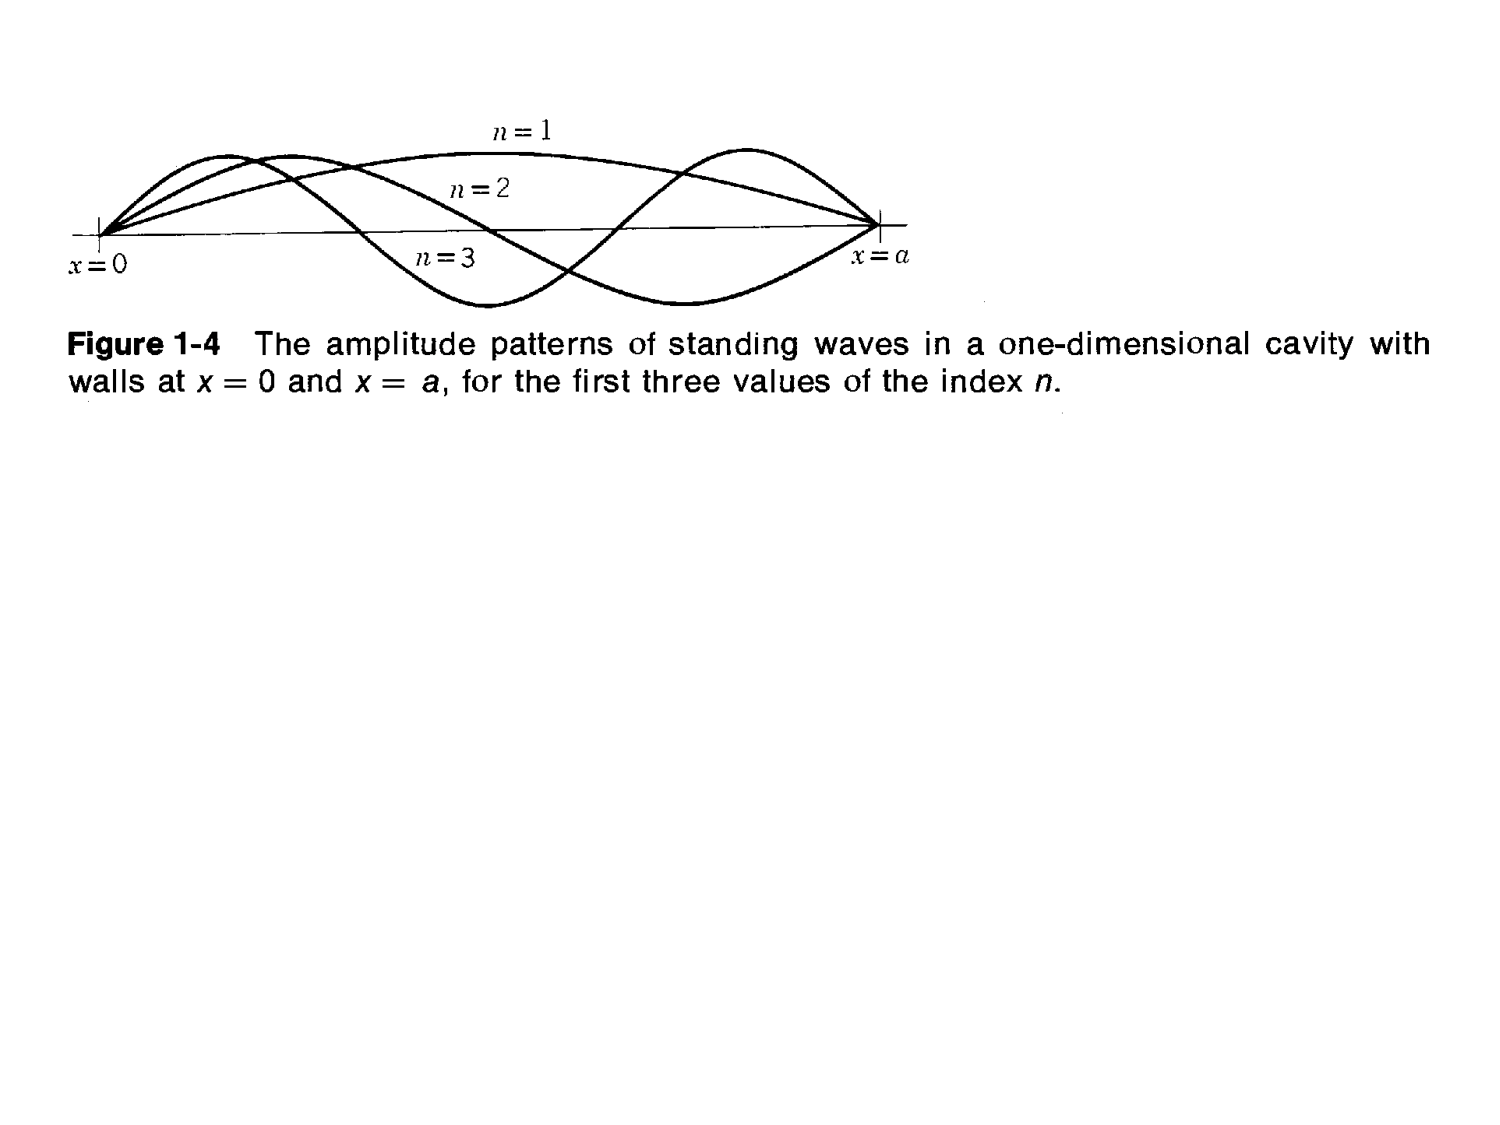
\includegraphics[scale=0.6]{/modiVibrazione}
\caption{modi vibrazione}
\end{figure}
\item Occorre contare il numero di onde, cominciamo dal caso 1-D lungo $x$
\begin{equation}
\begin{split}
& E(x, t) = E_0 \sin \Bigl(  \frac{2 \pi x}{\lambda}  \Bigr) \sin (2\pi \nu t) \\
& \frac{2x}{\lambda} = 0,1,2,3 ... = n \in \mathbb{N}
\end{split}
\end{equation}
Quindi $n=0$ corrisponde all'estremità, fissa, in $x=0$ e tutte le possibili onde stazionarie si trovano imponendo $x=a$:
\begin{equation}
\begin{split}
& \frac{ 2a}{\lambda } = n \quad\quad n = 1,2,3, ... \\
& \mbox{utilizzando la relazione} \quad \nu = \frac{c}{\lambda} \\
& \nu = \frac{ c n }{2a } \quad n = 1,2,3, ...
\end{split}
\end{equation}
Che sono quindi i valori permessi di frequenza per onde stazionarie.
\begin{figure}[h]
\centering
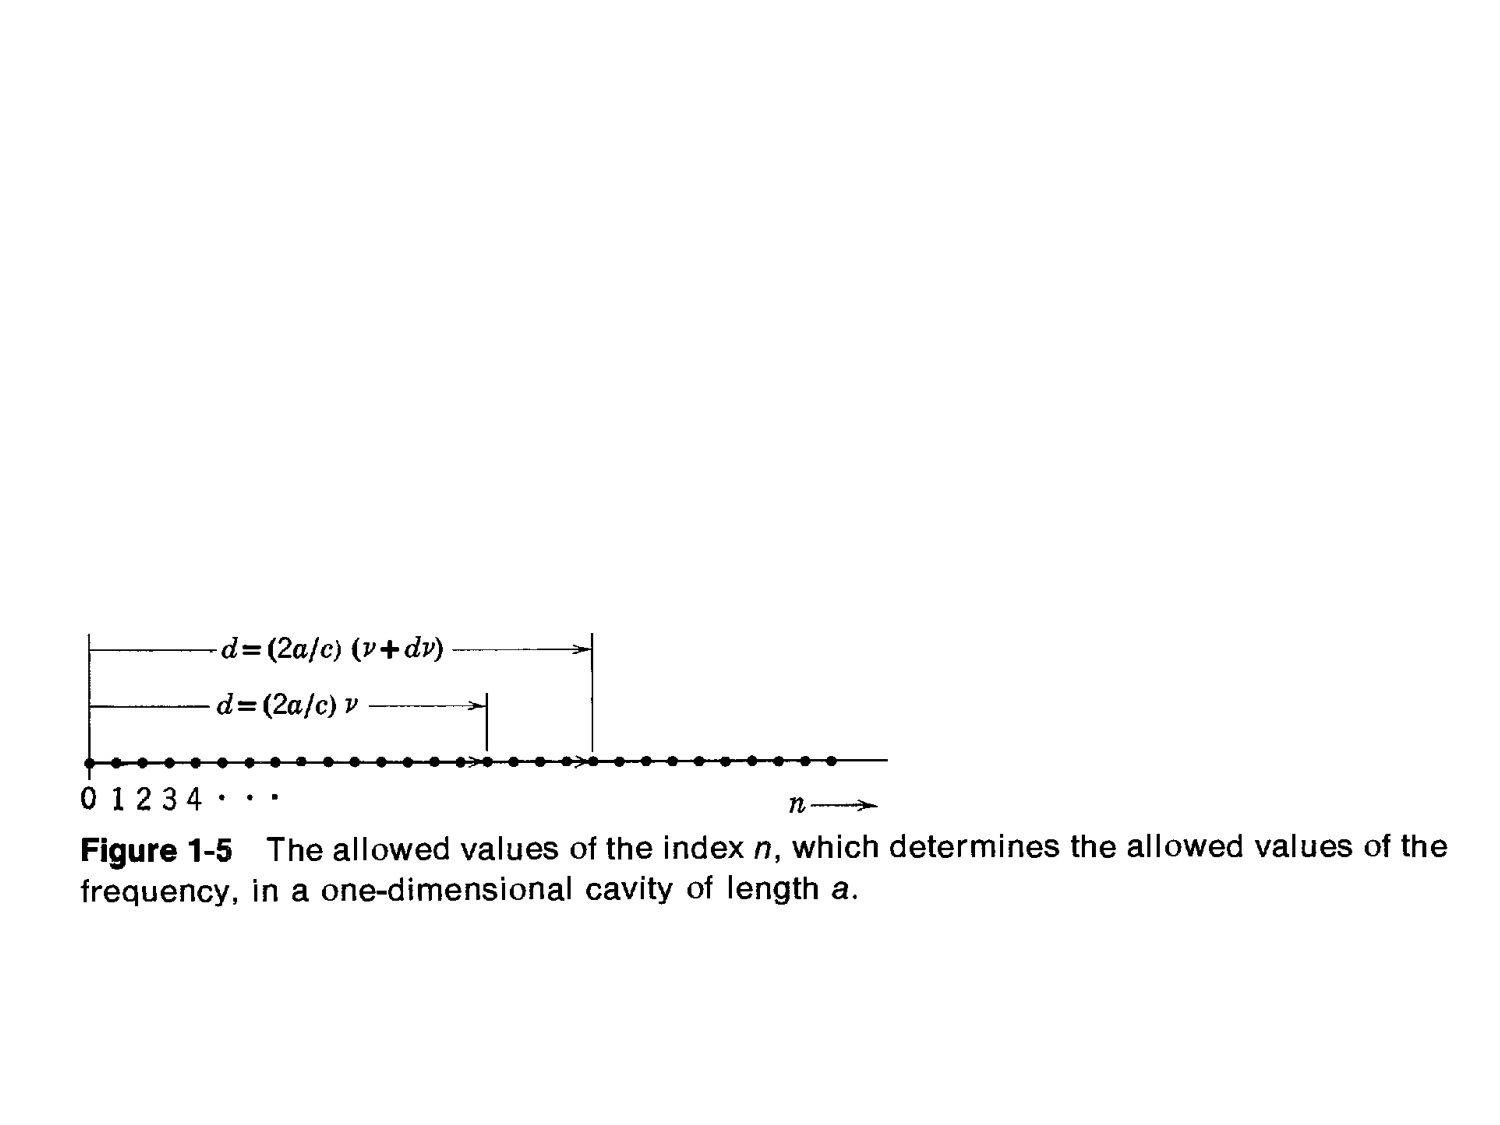
\includegraphics[scale=0.7]{/Blackbody_nodi}
\end{figure}
\begin{equation}
\begin{split}
& d = (\frac{ 2a}{c }) (\nu + d\nu) \quad - \quad d = (\frac{ 2a}{c }) \nu \\
& N(\nu)d\nu = 2 \Bigl(  \frac{2a}{c}  \Bigr) d\nu = \frac{4a}{c}d\nu 
\end{split}
\end{equation}
Nel caso unidimensionale questo è il numero di modi di vibrazione, dove il fattore 2 è dovuto al fatto che ci siano due possibili polarizzazioni $S$ e $P$. \\
\textbf{NB} Nel caso 1-D il numero di frequenze possibili non dipende da $\nu$.
Passiamo a 3 dimensioni, il valore di $n$ dipenderà ora da tre parametri $n_x, n_y, n_z \in \mathbb{N}$, da cui dipende anche il numero di frequenze permesse:
\begin{equation}
\begin{split}
& \frac{2a}{\lambda} = \sqrt{n_x^2 + n_y^2 + n_z^2} \\
& \nu = \frac{ c}{\lambda } = \frac{ c}{2a } \sqrt{n_x^2 + n_y^2 + n_z^2}
\end{split}
\end{equation}
\begin{figure}[h]
\centering
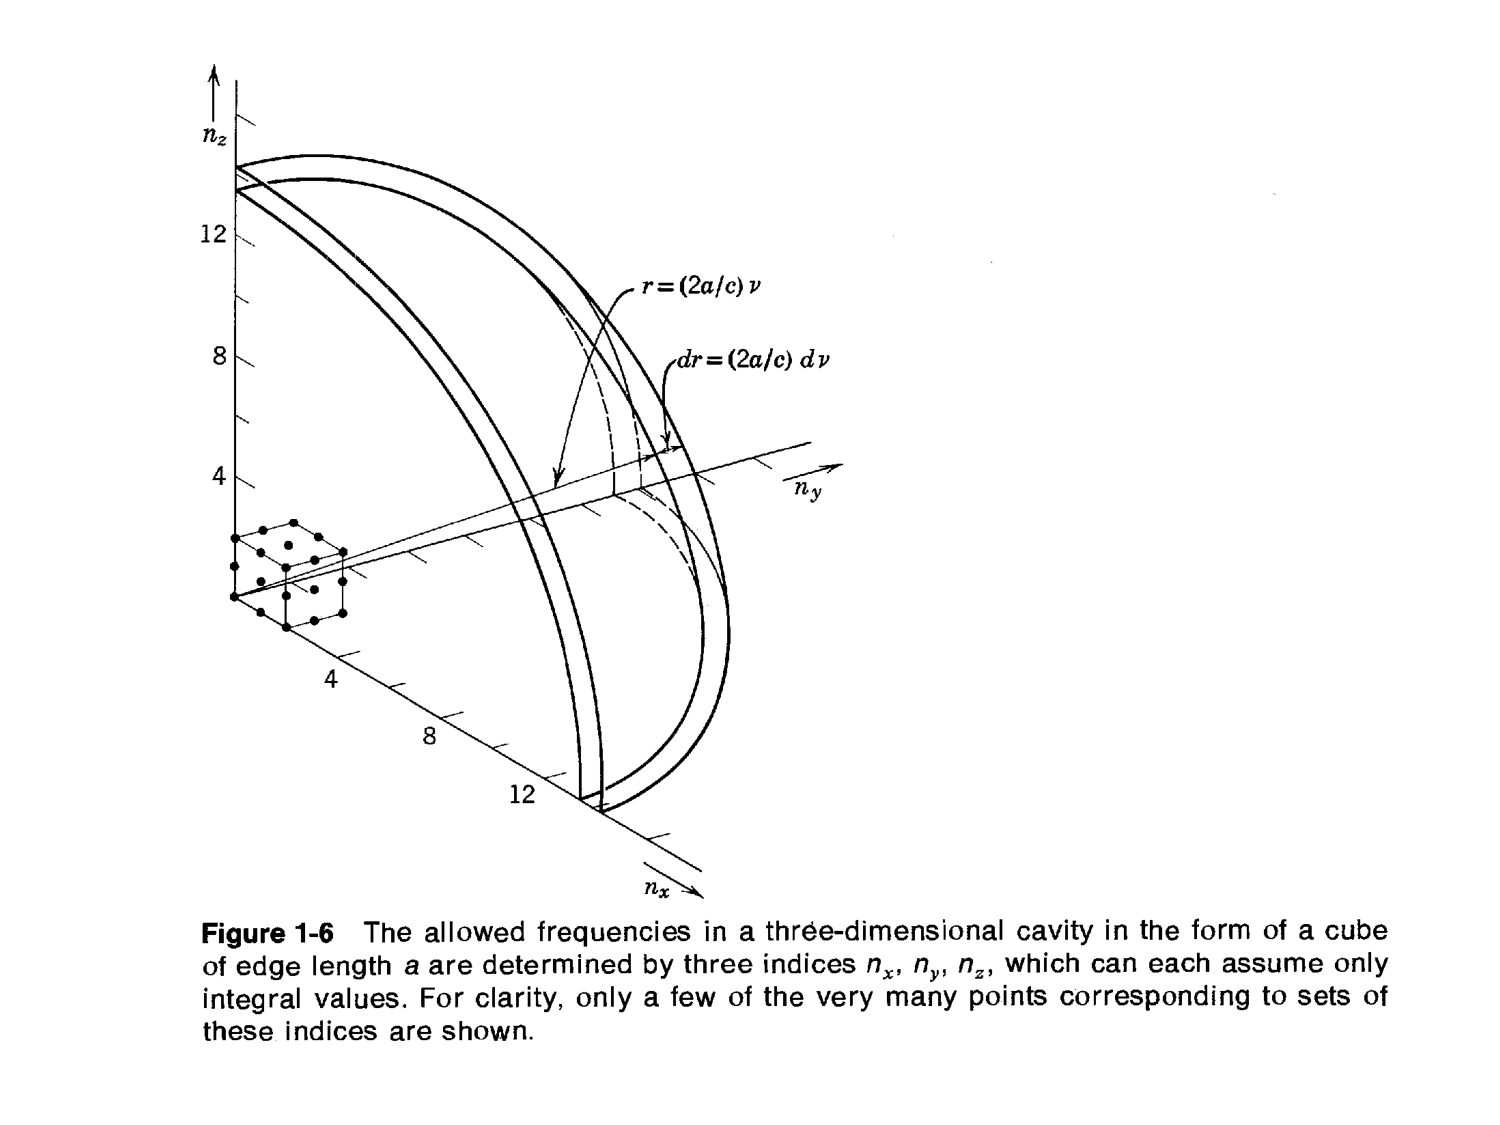
\includegraphics[scale=0.6]{/sfrera_nodi_permessi}
\caption{Numero di punti tra due shell a distanza $dr$, associati alle frequenze permesse}
\end{figure}
Conto quindi il numero di frequenze dal raggio $r$ al raggio $r + dr$:
\begin{equation}
\begin{split}
& N(\nu) d\nu = N(r)dr \\ 
& r = \frac{2a}{c}\nu \\
\end{split}
\end{equation}
ma il numero di punti nel volume dal raggio $r$ al raggio $r + dr$ è proprio il volume stesso, nel conto seguente utilizzo la sostituzione per $r$ appena trovata:
\begin{equation}
\begin{split}
& N(r) dr = \frac{ 1}{8 } 4 \pi r^2 dr = \frac{ \pi r^2 dr}{2 } \\
& N(\nu)d\nu = \frac{ \pi}{2 } \Bigl(  \frac{ 2a}{c }  \Bigr)^3 \nu^2 d\nu \\
& \mbox{che moltiplico x2 perché ho due stati di polarizzazione} \\
\Rightarrow & N(\nu) d\nu = \frac{ 8\pi V}{c^3 } \nu^2 d\nu
\end{split}
\end{equation}
ottengo così \underline{il numero di frequenze permesse} (modi di vibrazione) per le onde elettromagnetiche stazionarie all'interno della cavità di corpo nero, dove $V=a^3$ è il volume della cavità. \\
\textbf{NB} Nel caso 3-D il numero di frequenze possibili dipende da $\nu$.
\item Stima dell'energia media di ogni onda stazionaria di frequenza $\nu$.
Se ho un sistema di particelle in equilibrio termico, l'energia cinetica media per molecola per grado di libertà è data dalla \textbf{legge di equipartizione dell'energia}:
\begin{equation}
\begin{split}
\bar \varepsilon = \frac{ 1}{2 } & k_B T \\
\mbox{costante di Boltzmann } & k_B = \SI{1.3806e-23}{J/K}
\end{split}
\end{equation}
Considerando le onde come oggetti oscillanti devo tenere in considerazione anche l'energia potenziale, con argomentazioni di fisica classica, trovo l'energia media totale:
\begin{equation}
\bar \varepsilon = k_B T
\end{equation}
\end{enumerate}

\paragraph{Formula classica di Rayleigh Jeans per il corpo nero}
Moltiplicando il numero di onde stazionarie all'interno della cavità 
$$\frac{8 \pi \nu^2}{c^3}$$
per l'energia media di ogni onda stazionaria
$$k_BT$$
e dividendo per il volume $V$ si ottiene la \underline{densità di energia} $\rho_T(\nu)$ all'interno della cavità di corpo nero
\begin{equation}
\rho_T(\nu)d\nu = \frac{8 \pi \nu^2 k_B T }{c^3}d\nu
\end{equation}
La teoria classica di corpo nero è verificata solo per valori piccoli di $\nu$ e si discosta rapidamente dai dati sperimentali al crescere della frequenza, vedi figura \ref{catastrofeUV}.
\begin{figure}[h]
\centering
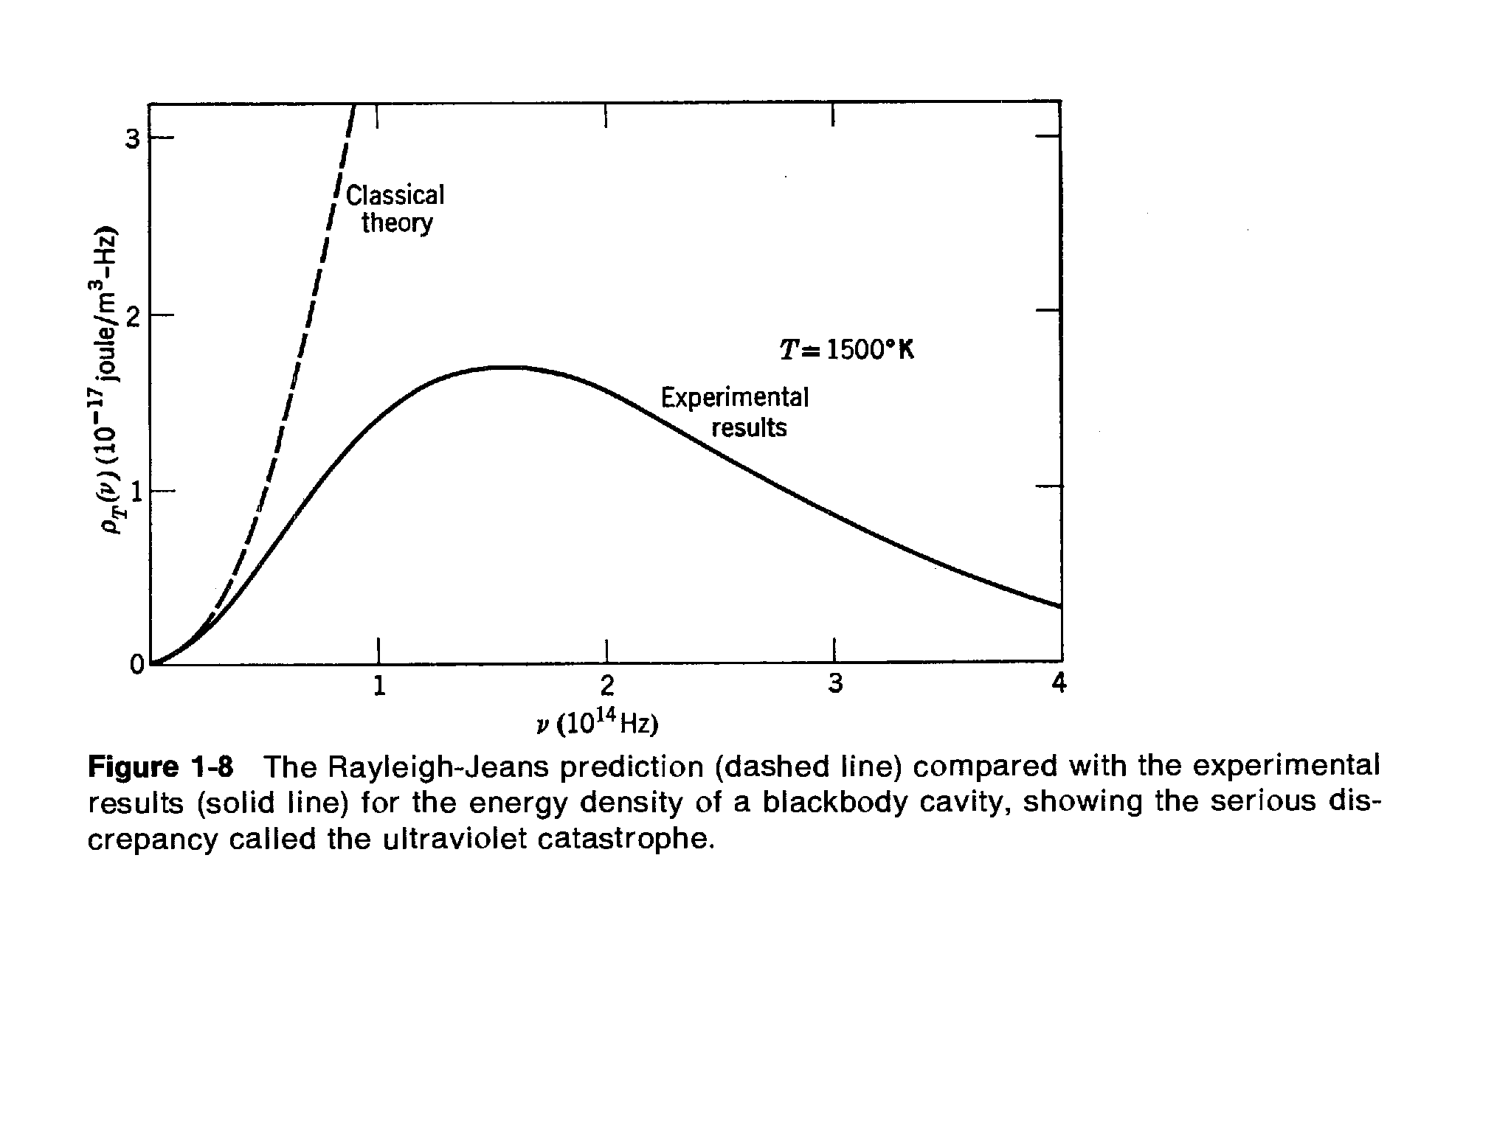
\includegraphics[scale=0.6]{/catastrofe_ultravioletta}
\caption{Catastrofe ultravioletta}
\label{catastrofeUV}
\end{figure}


\subsection{Statistica classica di Boltzmann}
Introduciamo la legge statistica classica di Boltzmann (o di Maxwell-Boltzmann) come la probabilità $P$ di trovare una certa entità di un sistema con energia nell'intervallo tra $\varepsilon$ e $\varepsilon+d\varepsilon$, data dalla formula
\begin{equation}
P(\varepsilon)d\varepsilon = C e^{ -\frac{\varepsilon}{k_BT } }
\end{equation}
Tale formula è valida quando il numero degli stati di energia \underline{non} dipende da $\varepsilon$, valida quindi ad esempio per l'oscillatore armonico unidimensionale.
La costante $C$ si calcola imponendo che l'integrale su tutto lo spettro di energie sia pari a $1$:
\begin{equation}
\begin{split}
\int_{0}^{\infty} P(\varepsilon) d\varepsilon & = C \int_{0}^{\infty} e^{ -\frac{\varepsilon}{k_BT } } d\varepsilon = 1 \\
C & = \frac{ 1}{k_BT }
\end{split}
\end{equation}
Per cui si trova la formula che descrive la statistica classica di Boltzmann 
\begin{equation}
P(\varepsilon) = \frac{ e^{ - \frac{\varepsilon}{k_BT } } }{k_BT }
\end{equation}

\paragraph{Applico la statistica di Boltzmann} agli elementi del set di onde stazionarie oscillanti nella cavità di corpo nero, quindi l'energia media è data da: 
a numeratore l'energia $\varepsilon$ moltiplicata (pesata) per la probabilità che l'entità abbia quell'energia (integrata su tutti i valori di energia), a denominatore ho la probabilità di trovare l'entità con qualsiasi energia (integrata su tutti i valori di energia), ponendo $\beta=\frac{1}{k_BT}$
\begin{equation}
\begin{split}
\bar\varepsilon & =\frac{\int_{0}^{\infty} \varepsilon P(\varepsilon)\,d\varepsilon}{\int_{0}^{\infty} P(\varepsilon)\,d\varepsilon} 
= \frac{\int_{0}^{\infty} \varepsilon \frac{ e^{ - \frac{\varepsilon}{k_BT } } }{k_BT } d\varepsilon}{\int_{0}^{\infty} \frac{ e^{ - \frac{\varepsilon}{k_BT } } }{k_BT }d\varepsilon}
= \frac{\int_{0}^{\infty} \varepsilon \beta e^{ - \beta \varepsilon } d\varepsilon}{\int_{0}^{\infty} \beta e^{ - \beta \varepsilon } d\varepsilon} \\
& = \frac{\int_{0}^{\infty} \varepsilon e^{ - \beta \varepsilon } d\varepsilon}{\int_{0}^{\infty} e^{ - \beta \varepsilon } d\varepsilon}
= - \frac{ d}{d\beta } \Bigl[  \ln \Bigl(  \int_0^{\infty} e^{ -\beta \varepsilon } d\varepsilon  \Bigr)   \Bigr]
= - \frac{ d}{d\beta } \Bigl(  \ln \frac{ 1}{\beta }  \Bigr) \\
& = \beta \frac{ 1}{\beta^2 } 
= \frac{ 1}{\beta } 
= k_BT
\end{split}
\label{energia_media_blackbody}
\end{equation}
Ottenendo così l'energia media di ogni onda stazionaria 
\begin{equation}
\bar \varepsilon = k_B T
\end{equation}
uguale al valore utilizzato da Rayleigh e Jeans e per cui si ha la catastrofe ultravioletta.


\subsection{Ipotesi quantica di Planck e formula di Planck per il corpo nero}
Planck ipotizza che l'energia non possa assumere qualsiasi valore ma solo valori discreti
$$\varepsilon = 0,\Delta\varepsilon,2\Delta\varepsilon,3\Delta\varepsilon, ...$$
Allora per misurare l'area del sottografico, e quindi la Radianza totale, non occorrerà più eseguire un integrale ma piuttosto una sommatoria su tutti i "rettangolini" discreti.
\begin{figure}[h]
    \centering
    \subfloat[Ipotesi quantica di Planck]{
        \label{ipotesi_quantica_Planck}
        \includegraphics[width=0.5\textwidth]{/ipotesi_quantica_Planck}
    }
    \subfloat[Sommatoria sui rettangolini del sottografico]{
        \label{rettangolini}
        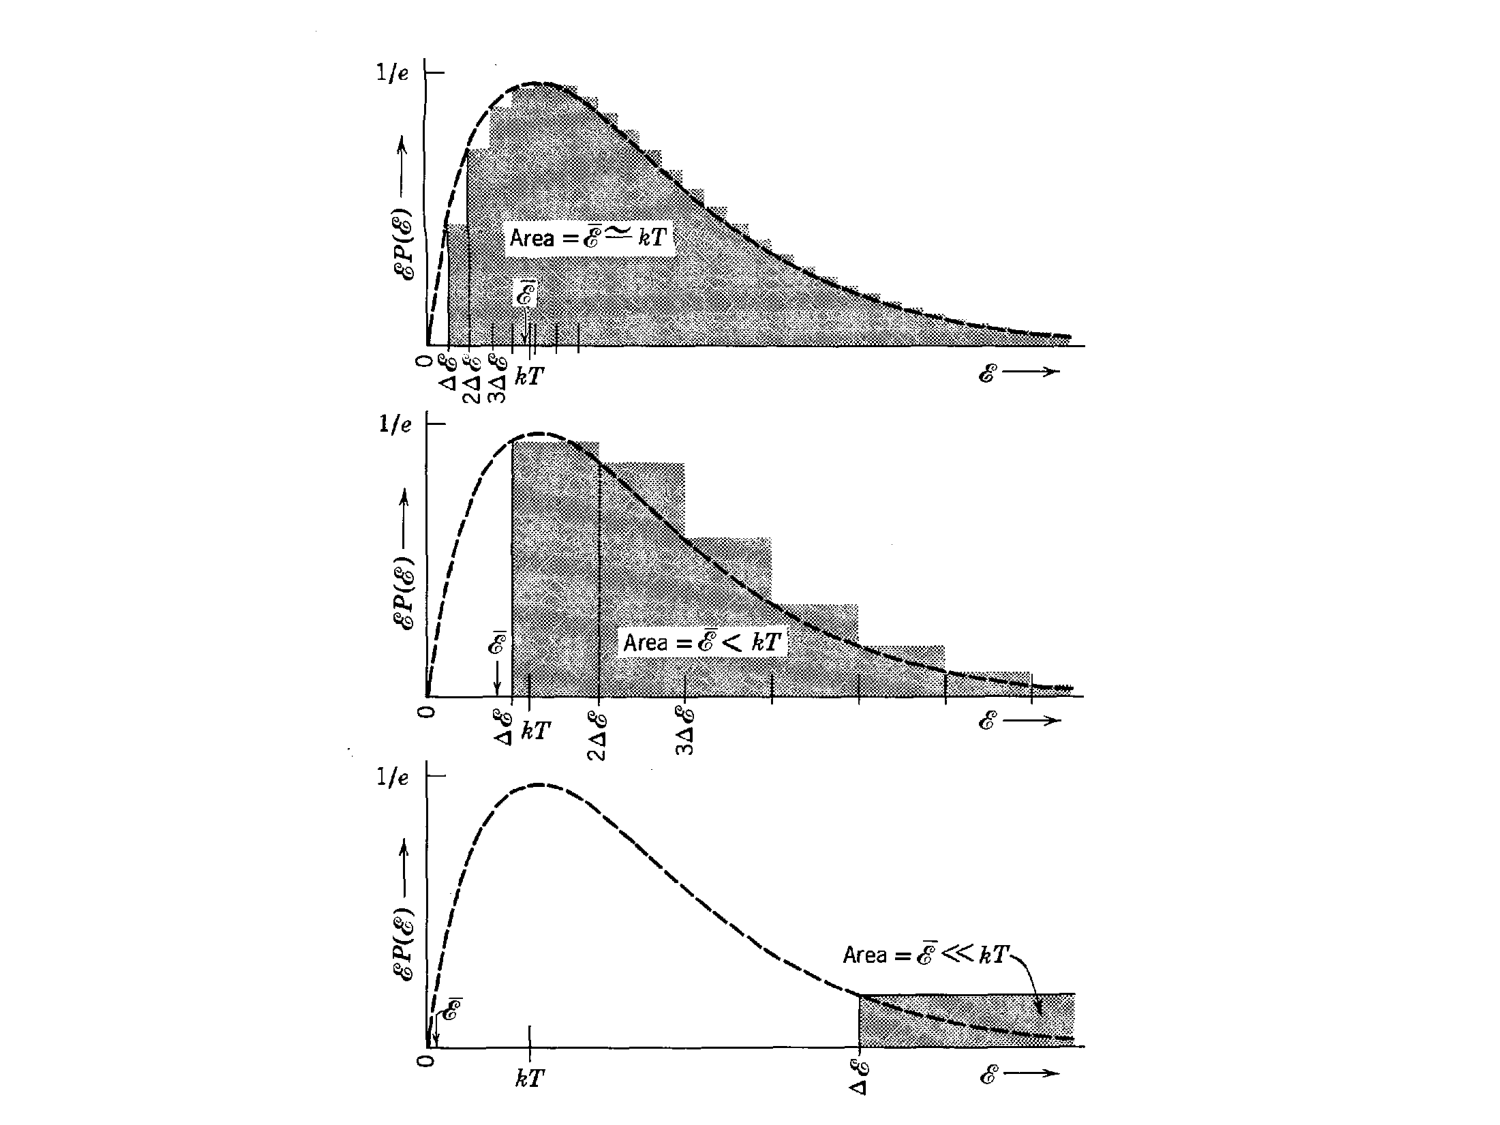
\includegraphics[width=0.5\textwidth]{/rettangolini}
    }
%    \caption{Overall_caption}
    \label{ipotesi_quantica_Planck_rettangolini}
\end{figure}
Analizzando l'andamento di $\bar\varepsilon$ in funzione di $\Delta\varepsilon$ si trova l'espressione:
\begin{equation}
\bar\varepsilon = \frac{ \Delta\varepsilon}{e^{ \frac{ \Delta\varepsilon}{k_BT } } - 1 }
\end{equation}
per cui i limiti di tale espressione sono
\begin{equation}
\begin{split}
& se \quad \Delta\varepsilon \rightarrow 0 \quad \Rightarrow \quad \bar\varepsilon \sim \frac{ 2 k_B^2 T^2 }{2kT + \Delta\varepsilon } \rightarrow k_BT  \quad \mbox{dove } e^x \sim 1 + x + \frac{ x^2}{2 } \\
& se \quad \Delta\varepsilon = k_BT \quad \Rightarrow \quad \bar\varepsilon = \frac{ k_BT }{ e - 1 } < k_BT \\
& se \quad \Delta\varepsilon \rightarrow \infty \quad \Rightarrow \quad \bar\varepsilon = \lim_{\Delta\varepsilon = \infty}  \frac{ \Delta\varepsilon}{e^{ \frac{ \Delta\varepsilon}{k_BT } } - 1 } = 0
\end{split}
\end{equation}
Quindi il risultato classico $\bar\varepsilon = k_BT$ è utile solo per $\Delta\varepsilon = h\nu \rightarrow 0$ ovvero per frequenze $\nu$ piccole.
La soluzione si trova se si mettono in correlazione $\Delta\varepsilon \propto \nu$ quindi scrivendo $\Delta\varepsilon = h\nu$ dove $h=\SI{6.63e-34}{J.s}$ è la Costante di Planck.
La \underline{quantizzazione dell'energia}, quindi i valori possibili dell'energia, si scrive come $n h \nu$ con $n = 0,1,2, ...$
L'espressione della probabilità $P(\varepsilon)$ è la legge statistica classica di Boltzmann in cui si sostituisce la relazione dell'energia $\varepsilon$ di Planck
\begin{equation}
\begin{split}
& P(\varepsilon) = \frac{ e^{ -\frac{ \varepsilon}{ k_BT} }}{k_BT }  \quad\quad \varepsilon= n h\nu \\
\bar\varepsilon & = \frac{ \sum_{n=0}^{\infty} \varepsilon P(\varepsilon)}{\sum_{n=0}^{\infty} P(\varepsilon) }
= \frac{ \sum_{n=0}^{\infty}  \frac{ nh\nu}{k_BT } e^{ -\frac{ nh\nu}{k_BT } }  }{\sum_{n=0}^{\infty} \frac{ 1 }{k_BT } e^{ -\frac{ nh\nu}{k_BT } } } \\
& = k_BT \frac{\sum_{n=0}^{\infty} n\alpha e^{ -n\alpha } }{\sum_{n=0}^{\infty} e^{ -n\alpha } } \quad\quad \alpha = \frac{ h\nu}{k_BT }
\end{split}
\end{equation}
si procede nel calcolo come nel caso classico, introducendo la seguente catena di uguaglianze
\begin{equation}
- \alpha \frac{ d}{d\alpha } \ln \sum_{n=0}^{\infty} e^{-n\alpha} = \frac{ - \alpha \frac{ d}{d\alpha } \sum_{0}^{\infty} e^{-n\alpha} }{ \sum_{0}^{\infty} e^{-n\alpha}} = 
\frac{ - \sum_{0}^{\infty} \alpha \frac{ d}{d\alpha } e^{-n\alpha} }{ \sum_{0}^{\infty} e^{-n\alpha}} = \frac{\sum_{0}^{\infty} n\alpha e^{ -n\alpha } }{\sum_{0}^{\infty} e^{ -n\alpha } }
\end{equation}
sostituendo si ottiene
\begin{equation}
\begin{split}
\bar\varepsilon = k_BT \Bigl(  - \alpha \frac{ d}{d\alpha } \ln \sum_{n=0}^{\infty} e^{ -n\alpha }  \Bigr) = -h\nu \frac{ d}{d\alpha } \ln \sum_{n=0}^{\infty} e^{ -n\alpha }
\end{split}
\end{equation}
utilizziamo ora la serie geometrica per eseguire la derivata
\begin{equation}
\sum_{n=0}^{\infty} e^{ -n\alpha } = 1 + e^{ -\alpha } + e^{ -2\alpha } + ... = 1 + x + x^2 + ... = \frac{ 1}{1-x } = \frac{ 1}{1- e^{- \alpha } }
\end{equation}
e si scrive il risultato come
\begin{equation}
\bar\varepsilon = - h\nu \Bigl[ - \frac{ e^{ -\alpha }}{1 - e^{ -\alpha } } \Bigr] = \frac{ h\nu}{ e^{ \alpha } - 1 } = \frac{ h\nu}{ e^{ \frac{ h\nu}{k_BT } } - 1} 
\end{equation}
quindi l'espressione finale dell'\textbf{energia media delle onde nella cavità} è
\begin{equation}
\bar\varepsilon = \frac{ h\nu}{ e^{ \frac{ h\nu}{k_BT }} - 1} 
\end{equation}
Per ottenere l'espressione della \underline{radiazione di cavità} moltiplico il numero di modi di vibrazione possibili per un'onda stazionaria all'interno della cavità
$$\frac{ 8\pi\nu^2}{c^3 }$$
per l'espressione dell'energia media di ogni onda stazionaria nella nuova ipotesi di Planck, ottengo quindi
\begin{equation}
\rho_T(\nu) d\nu = \frac{ 8\pi\nu^2}{c^3 } \frac{ h\nu}{ e^{ \frac{ h\nu}{k_BT }} - 1} d\nu
\end{equation}
anche detta \textbf{Formula di Planck per il corpo nero (1900)}, tale formula è in perfetto accordo con i dati sperimentali.
Questo risultato da inizio alla fisica moderna, introducendo il concetto di energia quantizzata inizia quindi la meccanica quantistica.
Cerchiamo ora un'espressione analoga in funzione di$\lambda$
$$\rho_T(\lambda) d\lambda = -\rho_T(\nu)d\nu $$
considero che
$$\nu = \frac{ c}{\lambda } \quad \Rightarrow \quad d\nu = -\Bigl(  \frac{ c}{\lambda^2 }  \Bigr) d\lambda \quad \Rightarrow \quad \frac{ d\nu}{d\lambda } = -\Bigl(  \frac{ c}{\lambda^2 }  \Bigr) $$
quindi sostituendo in questo modo
$$\rho_T(\lambda) = -\rho_T(\nu) \frac{ d\nu}{d\lambda } = -\rho_T(\nu) \frac{ c}{\lambda^2 }$$
si ottiene l'espressione cercata
\begin{equation}
-\rho_T(\lambda) d\lambda = \frac{ 8\pi h c }{\lambda^5 } \frac{ d\lambda}{e^{ \frac{ hc}{\lambda k_B T } } -1 }
\end{equation}
\begin{figure}[h]
\centering
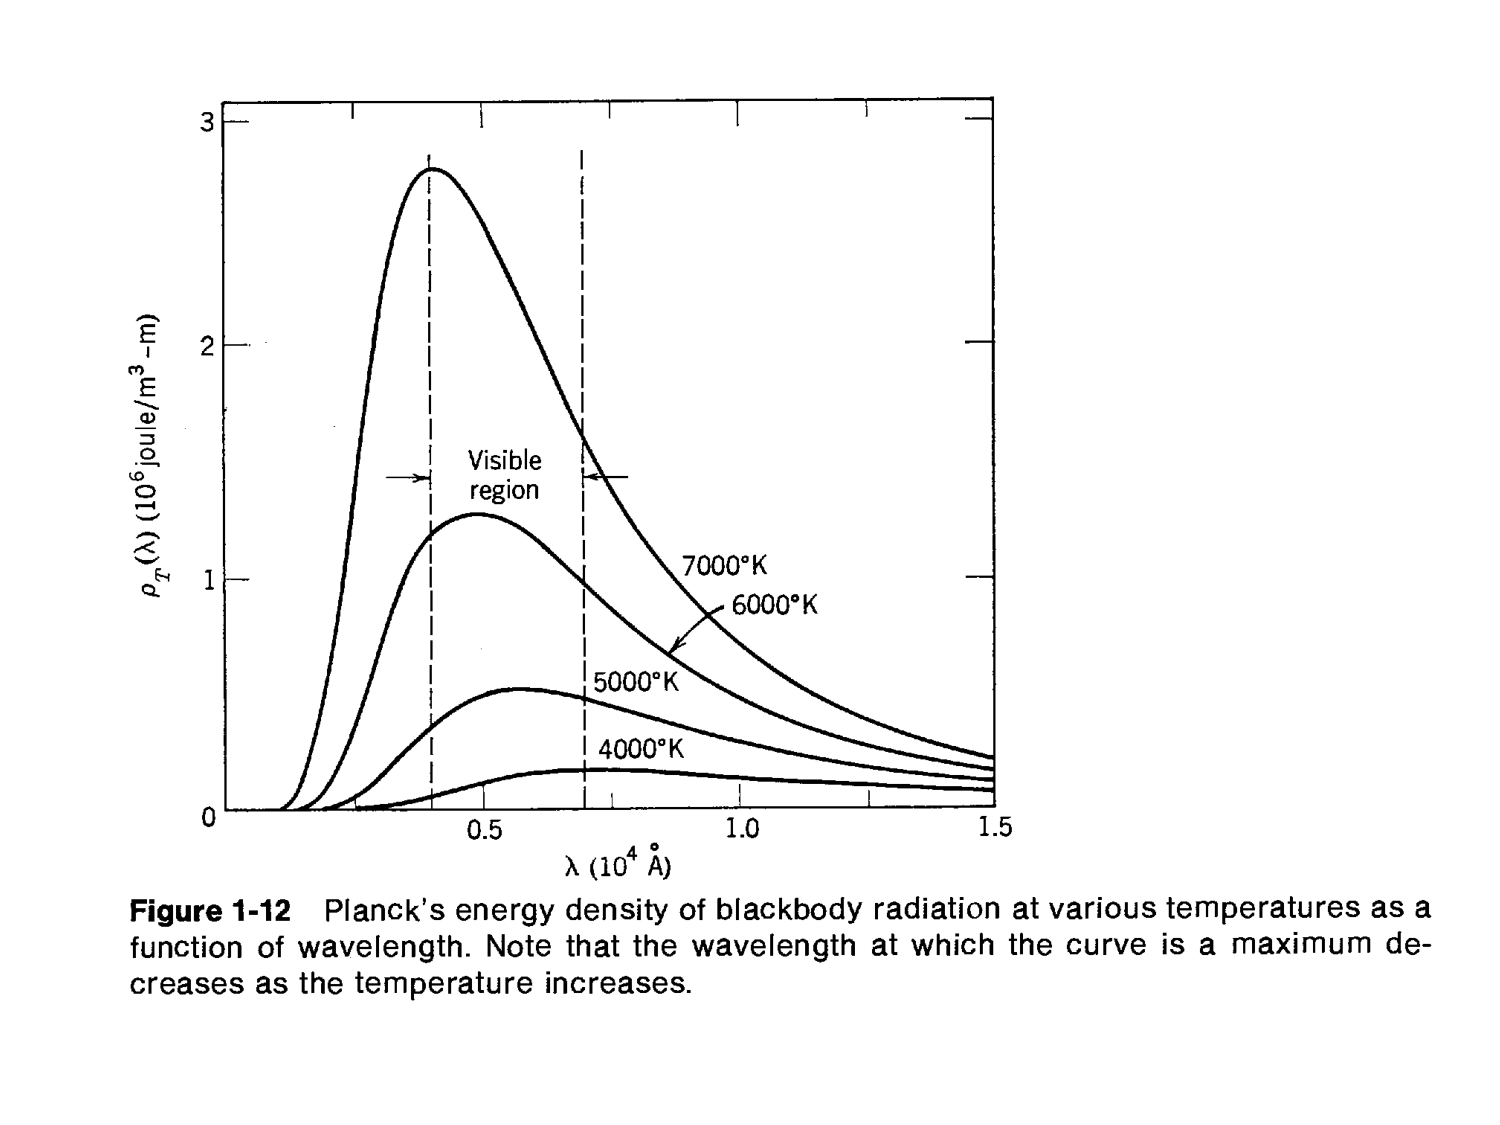
\includegraphics[scale=0.6]{/spettri_corponero}
\caption{Vari spettri di corpo nero}
\end{figure}

\paragraph{Postulato di Planck:} \textit{ogni entità fisica con un grado di libertà la cui "coordinata" è una funzione sinusoidale del tempo può avere solo energia totale $E$ tale che sia soddisfatta la relazione \\
$\varepsilon = n h \nu$ con $n=0,1,2, ...$ naturale.} \\
Il postulato di Planck si estende quindi a tutte le entità fisiche modellizzabili come oscillatori armonici semplici.
\begin{figure}[h]
\centering
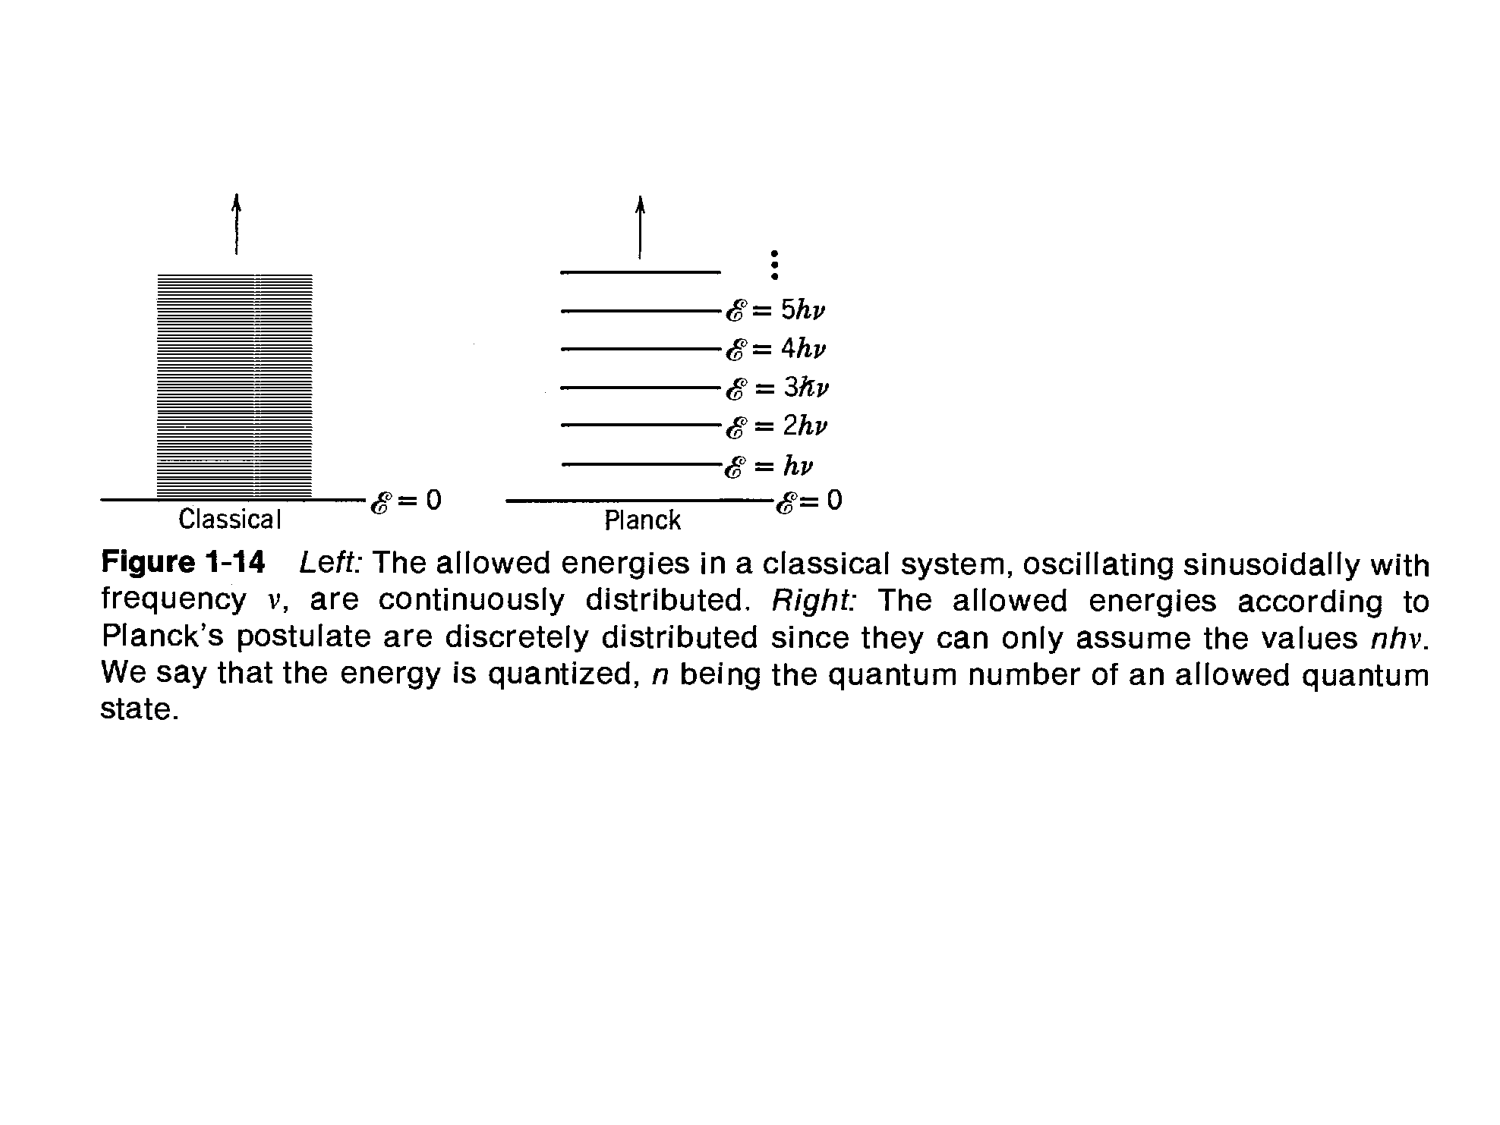
\includegraphics[scale=0.6]{/energia_quantizzata}
\caption{Confronto grafico tra la trattazione classica e quella quantizzata proposta da Planck}
\end{figure} 

\paragraph{Derivazione della legge di Stefan-Boltzmann}
Come si arriva alla formula di Stefan-Boltzmann partendo dalla formula di Planck per il corpo nero?
Ricordo che esiste le relazioni
$$\frac{ c}{4 } \rho_T(\nu) = R_T(\nu) \quad e \quad R_T = \int_0^{\infty} R_T(\nu)d\nu$$
quindi
\begin{equation}
\begin{split}
\rho_T(\nu) d\nu & = \frac{ 8\pi\nu^2}{c^3 } \frac{ h\nu}{ e^{ \frac{ h\nu}{k_BT }} - 1} d\nu \\
R_T &= \int_0^{\infty} \frac{ 2\pi h}{c^2 } \frac{ \nu^3}{e^{ \frac{ h\nu}{k_BT } } - 1 } d\nu \\
& = \frac{ 2\pi h}{c^2 } \Bigl(  \frac{ k_BT}{h }  \Bigr)^4 \int_0^{\infty} \frac{ x^3}{e^x - 1 }dx \quad \mbox{dove} \quad x=\frac{ h\nu}{k_BT }\\
\end{split}
\end{equation}
calcolo l'integrale noto
\begin{equation}
\int_0^{\infty} \frac{ x^3}{e^x - 1 }dx = \frac{ \pi^4}{15 }
\end{equation}
da cui ottengo il risultato finale 
\begin{equation}
R_T = \sigma T^4
\end{equation}
in cui compare la costante di Stefan Boltzmann
\begin{equation}
\sigma = \frac{ 2\pi^5 k_B^4}{15 h^3 c^2 } \simeq \SI{5.676e-8}{W / m^2 K^4}
\end{equation}

\newpage

\paragraph{Esercizio}
Si consideri una massa puntiforme $m=\SI{0.01}{kg}$ appesa ad un filo di lunghezza $l=\SI{0.1}{m}$ e sia $\theta=\SI{0.1}{rad}$ l'angolo massimo di oscillazione. L'energia di questo pendolo appare continua o quantizzata? \\
\underline{Soluzione:}
utilizzando risultati di fisica classica, calcolo la frequenza di questo pendolo
\begin{equation}
\nu = \frac{ 1}{2\pi } \sqrt{\frac{ g}{l }} = \frac{ 1}{2\pi }\sqrt{\frac{ \SI{9.81}{m/s^2}}{\SI{0.1}{m} }} = \SI{1.6}{Hz}
\end{equation}
e calcolo l'energia potenziale del pendolo
\begin{equation}
mgh = mgl(1-\cos \theta) = \SI{0.01}{kg} \cdot \SI{9.81}{m/s^2} \cdot \SI{0.1}{m} \cdot (1-\cos \theta) = \SI{5e-5}{j}
\end{equation}
Il quanto di energia che posso associare a questo pendolo 
\begin{equation}
\Delta E = h\nu = \SI{6.63e-34}{j.s} \cdot \SI{1.6}{Hz} = \SI{e-33}{j}
\end{equation}
nell'ipotesi che l'energia del pendolo sia quantizzata.
Ottengo un numero molto piccolo rispetto all'energia complessiva del pendolo, per cui il rapporto
\begin{equation}
\frac{ \Delta E }{E } = \SI{2e-29}{}
\end{equation}
Possiamo renderci conto della quantizzazione solo quando il quanto $\Delta E$ e l'energia $E$ sono grandezze confrontabili.
Da cui si vede come la fisica classica offra un'ottima approssimazione per lo studio di problemi di questo tipo.


